% !TEX encoding = UTF-8 Unicode

\documentclass[twocolumn,10pt,a4j]{ltjsarticle}
\usepackage{kougai}

\title{ゲームに最適化されたベンチマークソフト「FlexBench」開発}
\author{2032087 大司 陽輝  指導教員 須田 宇宙 准教授}
\date{}

\begin{document}

\maketitle

\section{はじめに}
コンピューターゲームは50年前から没入感を得るために進化してきた.具体的には,ゲーム画面の解像度が向上し,キャラクターや背景が物理法則に則って動くようになった.このような処理を行うためにCPUやGPUが発展し,高性能なゲーミングPCが注目された.しかし,プレイしたいゲームに対応したゲーミングPCの購入や,パーツの選定は難しい.その要因は,現状のベンチマークソフトにある.
そこで本研究ではゲームタイトルごとの処理を模したベンチマークソフトの開発を行う.

\section{既存のベンチマークでは}
ゲーム内で没入感を高める上で,高解像度化や,質感を高めるために草木を動かす処理や,キャラクターを動かすための処理が行われており,ゲームタイトルごとに処理内容は異なる.
既存のベンチマークではCPUやGPUの性能を計ることは可能であるが,ゲームタイトルごとの処理に則していない.
その結果,現状のベンチマークでは,適切な評価が得られない.
 
\section{処理に時間がかかる内容}
 \subsection{GPUの処理について}
ゲーム内では草木を動かす処理や,質感を高めるために個別の小さなプログラムが扱われている.それらのプログラムはシェーダーと呼ばれている.
ゲーム内ではシェーダーが数十〜数百の処理がされている.
図1は,解像度の違いによる没入感の違いを表したものであり,画面中央から左側が192x108,右側が1920x1080の解像度となっている.図1のように解像度を向上させると,没入感を得ることができるが,向上に伴ってGPUへの負荷のかかり方も変動する.
\begin{figure}[h]
\begin{center}
 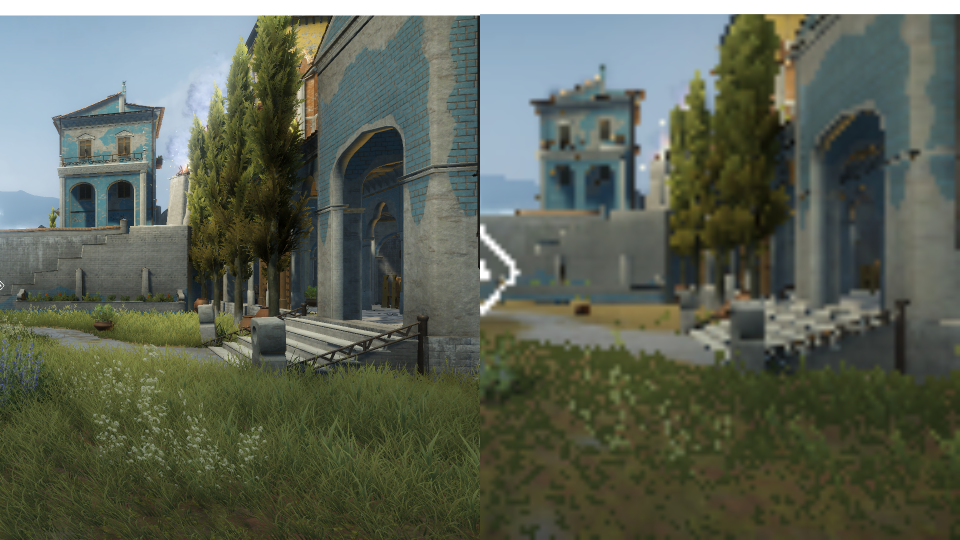
\includegraphics[clip,width=85mm,height=45mm]{picture_1.png}
  \end{center}
 \caption{解像度の違い}
 \label{fig:教科書}
\end{figure}

  \subsection{CPUの処理について}
  ゲーム内ではプレイヤーに対応したNPCの行動の処理や,物体の重力の物理演算などが行われている.
  NPCの行動の複雑さや,処理を行う物体の数に応じてCPUの処理性能が変動する.

\section{実装}


\section{開発したベンチマークソフトからわかったこと}

\section{やること・やったこと}

論文や書籍から,ゲームで行われるグラフィックなどの処理を学び,開発を行うベンチマークソフトの参考とする.


\section{今後の予定}
Unityで,ゲームと同様の処理を行えるソフトの開発を行う

\begin{thebibliography}{99}
\bibitem{1} 須田宇宙: ``音響科学e-Learning教材'', \url{https://www.youtube.com/watch?v=rZdvL0ju4CA&ab_channel=TheSpyHood}, 2018/7/19参照
\end{thebibliography}

\end{document}
